% !TeX spellcheck = en_US
\section{Problem 4}

In this problem, we are asked to write a program that implements backpropagation algorithm for an $1 - S^1 - 1$ network with $S^1=\left\{2,8,12\right\}$, as shown in figure~\ref{fig:prob4_nns}.

The first layer has $logsig$ as activation function and the output layer has $ReLU$ as activation function. Also, every weight and bias is initialized to a uniformly random number in $\left(-0.5, 0.5\right)$.
All of the above are done in order to train our network to approximate the following function:
\[
g(p) = 1 + e^{p\left(\dfrac{3\pi}{8}\right)}, \qquad p \in \left[-2,2\right]
\]

This means that, during training, we have to train the network for multiple input data (\textit{specifically, for all input data}).

\begin{figure}[H]
	\centering
	\begin{subfigure}{0.47\textwidth}
		\centering
		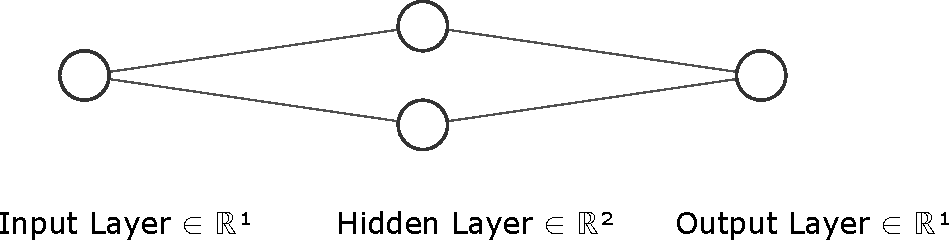
\includegraphics[width=0.9\textwidth]{../Problem 4/nn_1_2_1.pdf}
		\caption{$S^1=2$}
	\end{subfigure}
	\begin{subfigure}{0.47\textwidth}
		\centering
		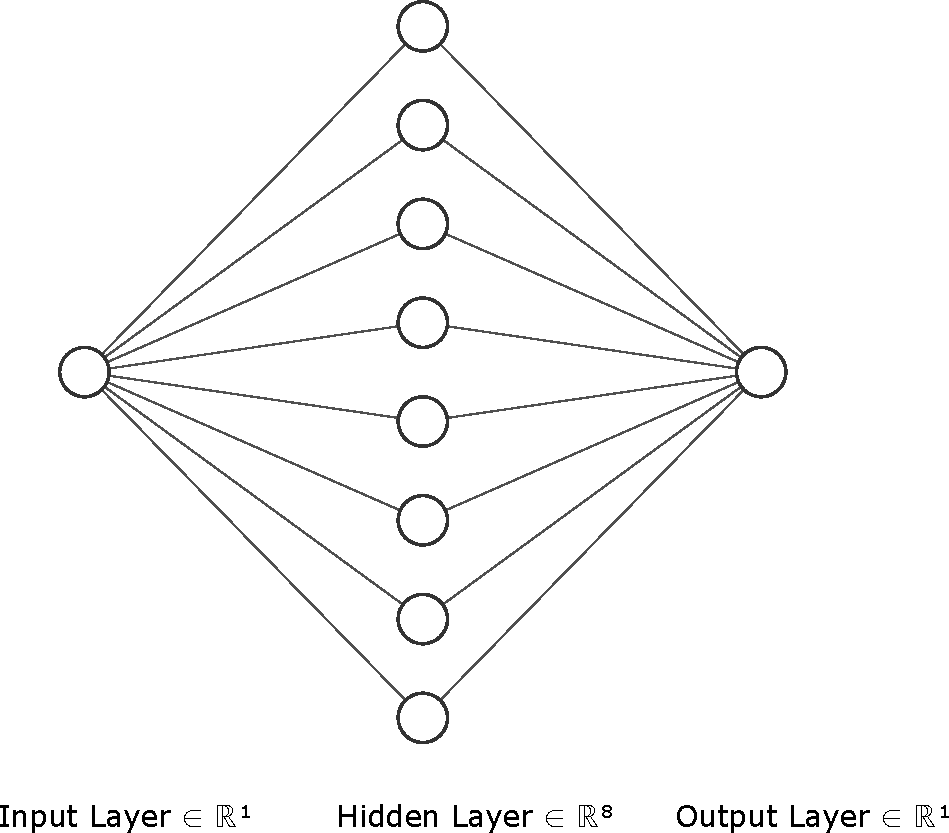
\includegraphics[width=0.9\textwidth]{../Problem 4/nn_1_8_1.pdf}
		\caption{$S^1=8$}
	\end{subfigure}
	\begin{subfigure}{0.47\textwidth}
		\centering
		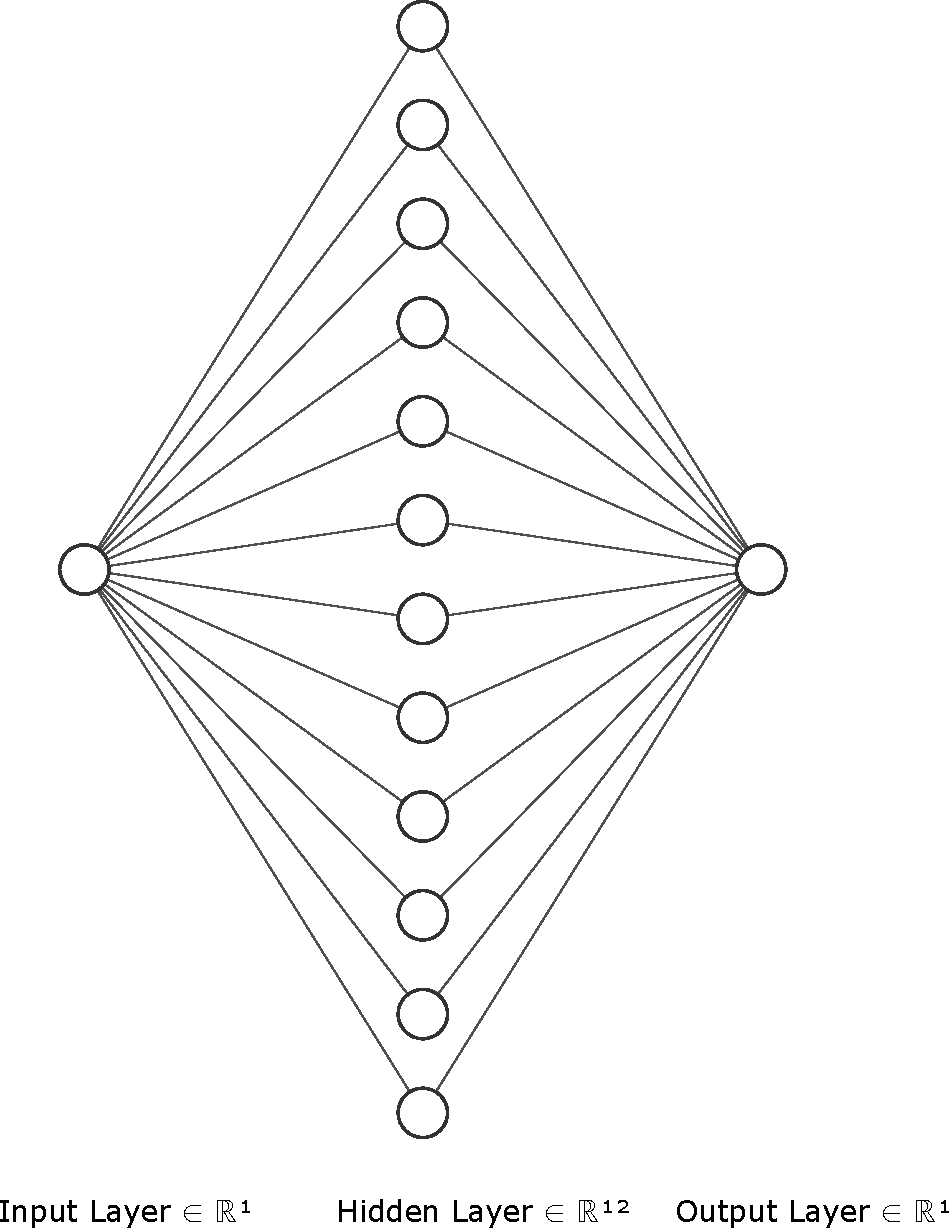
\includegraphics[width=\textwidth]{../Problem 4/nn_1_12_1.pdf}
		\caption{$S^1=12$}
	\end{subfigure}
	\caption{All the neural networks in this problem.}
	\label{fig:prob4_nns}
\end{figure}

We chose to write this program in MATLAB, despite the majority of these problems being written in Python. This ensures that we are going to use matrix operations for initialization of all weights and biases, as the problem .
The file \say{\textit{backpropagation.m}} contains all of the necessary code.\\

In order to see what difference $S$ and learning rate does to our network, we defined the following learning rates $\left[0.1, 0.01, 0.001\right]$ and generated the network's output and error throughout training.

%From the first view, we can see in figure~\ref{fig:prob4_1_2_1_failed_attempt} that 
From the very first run ($S=2,\ \alpha=0.001$), we can see in figure~\ref{fig:prob4_1_2_1_failed_attempt} that the back-propagation algorithm didn't converge at all, keeping the error to a constant value throughout the epochs.

\begin{figure}[htpb]
	\centering
	\begin{subfigure}{0.47\textwidth}
		\centering
		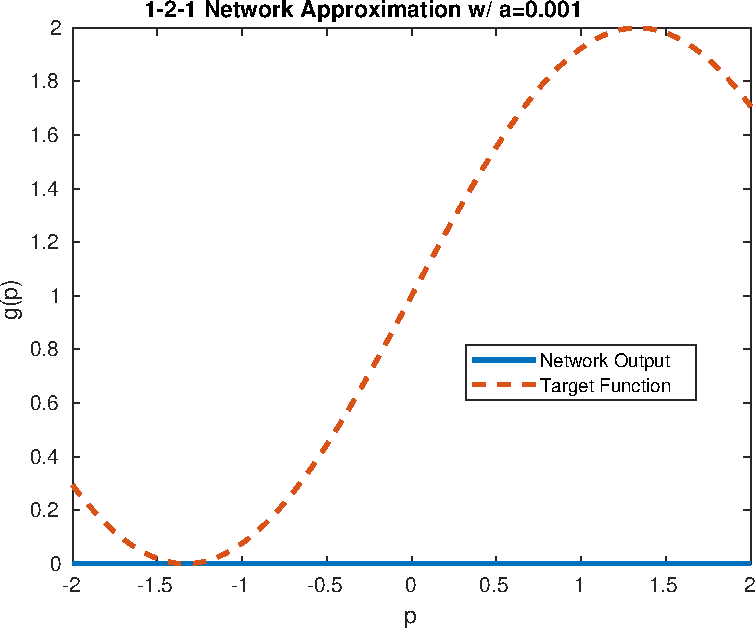
\includegraphics[width=\textwidth]{../Problem 4/1_2_1_failed_approximation.pdf}
		\caption{Approximation of input signal}
	\end{subfigure}
	\begin{subfigure}{0.47\textwidth}
		\centering
		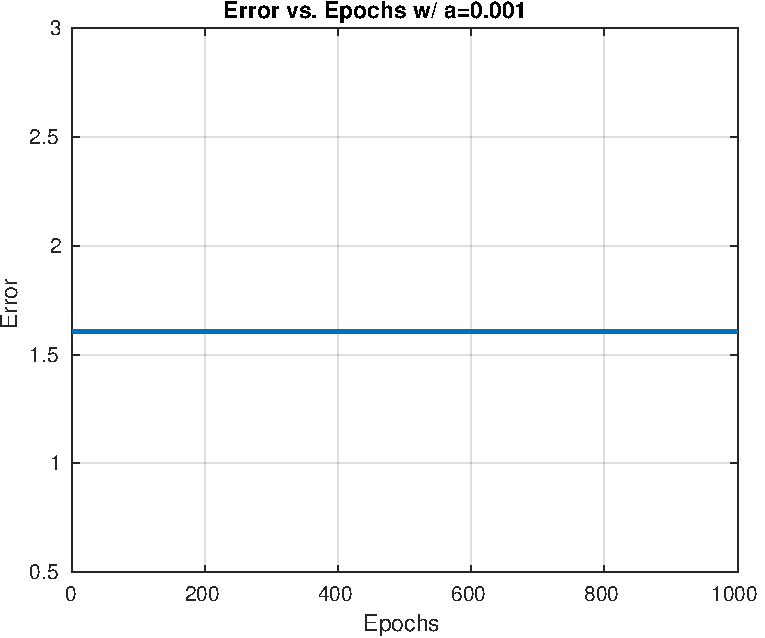
\includegraphics[width=\textwidth]{../Problem 4/1_2_1_failed_approximation_error.pdf}
		\caption{Error over iterations}
	\end{subfigure}
	\caption{A failed attempt of approximating the input signal. \\ The reason this approximation failed derives from the uniformly random initial guess for the weights and biases.}
	\label{fig:prob4_1_2_1_failed_attempt}
\end{figure}